\documentclass[xcolor={dvipsnames,usenames}]{beamer}
%\documentclass[xcolor={dvipsnames,usenames},handout]{beamer} % use this to compile w/o pauses
\mode<presentation>
{
\usetheme{madrid}
\usecolortheme{default}
\setbeamertemplate{itemize items}[default]
\setbeamertemplate{enumerate items}[default]
\setbeamercovered{transparent}
\usefonttheme[onlymath]{serif}
}


\usepackage{microtype}
\usepackage[normalem]{ulem}
%\usepackage{hyperref}
%\hypersetup{colorlinks=true, urlcolor=Blue, citecolor=Green, linkcolor=BrickRed, breaklinks, unicode}

\usepackage[nocompress]{cite}
\usepackage{amsmath,mathtools,stmaryrd}
\usepackage{enumerate}
\usepackage{latexsym,amsmath}
\usepackage{amssymb,stmaryrd}
\usepackage{euscript}
\usepackage{algorithm,algorithmicx}
\usepackage[noend]{algpseudocode}
\renewcommand{\algorithmicrequire}{\textbf{Requirement:}}

\usepackage{mathtools} % for \coloneqq

\usepackage{graphicx}
\usepackage{epstopdf}
\usepackage{subcaption}
\graphicspath{{./fig/}}


\title{Approximate Minimum-Weight Partial Matching under~Translation}
\author[Allen Xiao]
{
	Pankaj~Agarwal \inst{1} \and
	Haim~Kaplan \inst{2} \and
	Geva~Kipper \inst{2} \and
	Wolfgang~Mulzer \inst{3} \and
	G{\"u}nter~Rote \inst{3} \and
	Micha~Sharir \inst{2} \and
	Allen~Xiao \inst{1}
}
\institute[ISAAC 2018]
{
	\inst{1} Duke University \and
	\inst{2} Tel Aviv University \and
	\inst{3} Freie Universit{\"a}t Berlin
}
\date{December 2018}

% tweak wd=X\paperwidth to modify the footer dimensions in the madrid theme
\makeatletter
\setbeamertemplate{footline}{
  \leavevmode%
  \hbox{%
  \begin{beamercolorbox}[wd=.25\paperwidth,ht=2.25ex,dp=1ex,center]{author in head/foot}%
    \usebeamerfont{author in head/foot}\insertshortauthor\expandafter\ifblank\expandafter{\beamer@shortinstitute}{}{~~(\insertshortinstitute)}
  \end{beamercolorbox}%
  \begin{beamercolorbox}[wd=.55\paperwidth,ht=2.25ex,dp=1ex,center]{title in head/foot}%
    \usebeamerfont{title in head/foot}\insertshorttitle
  \end{beamercolorbox}%
  \begin{beamercolorbox}[wd=.2\paperwidth,ht=2.25ex,dp=1ex,right]{date in head/foot}%
    \usebeamerfont{date in head/foot}\insertshortdate{}\hspace*{2em}
    \insertframenumber/\inserttotalframenumber \hspace*{2ex}
  \end{beamercolorbox}}%
  \vskip0pt%
}
\makeatother


% make tables less packed
\renewcommand{\arraystretch}{1.5}
% get rid of caption labels
%\setbeamertemplate{caption}{\raggedright\insertcaption\par}
%\captionsetup[subfigure]{labelformat=empty}
% set beamer highlight color (alert)
\setbeamercolor{alerted text}{fg=BrickRed}

\newcommand{\mycite}[1]{{\color{LimeGreen}\lbrack #1\rbrack}}
\newcommand{\etal}{\textit{et~al.}}
\newcommand{\softO}{\widetilde{O}}
\newcommand{\reals}{\mathbb{R}}
\newcommand{\ints}{\mathbb{N}}
\newcommand\nats{\mathbb{N}}
\newcommand{\eps}{\varepsilon}
\DeclareMathOperator{\polylog}{polylog}
\DeclareMathOperator{\poly}{poly}
\newcommand{\flr}[1]{{\lfloor #1\rfloor}}
\DeclareMathOperator*{\argmax}{arg\,max}
\DeclareMathOperator*{\argmin}{arg\,min}
\DeclareMathOperator{\Vor}{Vor}
\DeclareMathOperator{\VorRegion}{VorRegion}

\def\abs#1{\mathopen| #1 \mathclose|}		% use instead of $|x|$
\def\norm#1{\mathopen\| #1 \mathclose\|}	% use instead of $\|x\|$

\DeclareMathOperator{\cost}{cost}
\newcommand{\tsupply}{\lambda}
\newcommand{\fsupply}{\phi}

\newcommand{\A}{{\color{red}A}}
\newcommand{\B}{{\color{blue}B}}
\newcommand{\M}{\EuScript{M}}
\newcommand{\tildeM}{\widetilde{\EuScript{M}}}
\newcommand{\X}{\EuScript{X}}

%\def\EMPH#1{\textcolor{BrickRed}{{\emph{#1}}}}



\begin{document}


\begin{frame}
\maketitle
\end{frame}


% outline
% problem demonstration, refer to static problem
% formal statements: 
%	l_p cost function, 
%	P1: find the optimal translation, and 
%	P2: complexity (no. faces) of the minimization diagram
% 	studied previously for p=2 (rms), but even for p=2 whether M is polynomial is open
%	best bound for p=2: O(n^2m^3.5 (e\ln m + e)^m)
% results:
% 	P2: polynomial complexity approximate diagram
%	P1: polytime approximation algorithm after constructing approx. diagram
% outline for approx diagram:
%	Lipschitz continuity for cost() under any l_p cost
%	given that, point-to-point translations (Cabello et al.) are a constant approx.
%	tile cells with an \eps-grid (also Cabello et al.) to improve to (1+\eps)
%	reduced set of centers: greedy disk eating
% algorithm for P1: apply a stationary k-matching algorithm to each center
% state Lipschitz property (calculation?)
% point-to-point translations and constant approx
% eps-grid tiling
% smaller set of centers


%SECTION: pmt

% gentle example + equation
\begin{frame}{Example}
% point sets A and B of size m, n respectively
% allowed to translate A --> A+t
% minimum-cost k-matching between A+t and B
% what's the best translation?
\begin{figure}
\begin{center}
\includegraphics<1>[width=\textwidth,page=1]{pmt_example}%
\includegraphics<2>[width=\textwidth,page=2]{pmt_example}%
\includegraphics<3>[width=\textwidth,page=3]{pmt_example}%
\includegraphics<4>[width=\textwidth,page=4]{pmt_example}%
\includegraphics<5>[width=\textwidth,page=5]{pmt_example}%
\includegraphics<6>[width=\textwidth,page=6]{pmt_example}%
\includegraphics<7->[width=\textwidth,page=7]{pmt_example}%
\end{center}
\end{figure}
\begin{itemize}
\item<7-> Find the minimum-cost matching over all translations.
% in words, mention polytime algorithms when t fixed ``well studied problem''
\end{itemize}
\end{frame}

% introduce cost function, ``second main question involves the structure of the cost function''
\begin{frame}{Cost function}
% equation
% static problem (t fixed) has polytime algorithms, e.g. Hungarian algorithm [RT]
\begin{itemize}
\item Given point sets $A$, $B$, with $|A| = m$ and $|B| = n$, match $A$ into an $m$-subset of $B$ after translation $t$.
\item For matching $M$ and translation $t$, define the \alert{root-mean-sqaure (RMS) cost} of the matching:
	\begin{equation*}
	\cost(M, t) \coloneqq \left[\frac{1}{m}\sum_{(a, b) \in M}\norm{a+t-b}^2\right]^{1/2}
	\end{equation*}
%\pause
%\item Can generalize to $p$-th power/$p$-th root, and matching of size $k$.
\pause
\item Best matching cost at each translation:
	\begin{equation*}
	\cost^*(t) \coloneqq \min_{\text{matching $M$}} \cost(M, t)
	\end{equation*}
\end{itemize}
\end{frame}

% cost under perturbations
\begin{frame}{Cost function under perturbations}
% equation
% figures through: small perturbation, larger perturbation, general question
\begin{equation*}
\cost^*(t) \coloneqq \min_{\text{matching $M$}} \cost(M, t)
\end{equation*}
\begin{figure}
\begin{center}
\includegraphics<1>[width=0.7\textwidth,page=8]{pmt_example}%
\includegraphics<2>[width=0.7\textwidth,page=9]{pmt_example}%
\includegraphics<3>[width=0.7\textwidth,page=10]{pmt_example}%
\includegraphics<4>[width=0.7\textwidth,page=11]{pmt_example}%
\includegraphics<5->[width=0.7\textwidth,page=12]{pmt_example}%
\end{center}
\end{figure}
\begin{itemize}
\item<6-> How many distinct matchings appear in $\cost^*(t)$?
\end{itemize}
\end{frame}

% minimization diagram M
\begin{frame}{How many distinct matchings? (1-dimensional)}
% function over t for each k matching
% cost*(t): the lower envelope
% vertical projection subdivides the plane
\begin{equation*}
\cost^*(t) \coloneqq \min_{\text{matching $M$}} \cost(M, t)
\end{equation*}
\begin{figure}
\begin{center}
\includegraphics<1>[width=0.6\textwidth,page=1]{lower_env}%
\includegraphics<2>[width=0.6\textwidth,page=2]{lower_env}%
\includegraphics<3>[width=0.6\textwidth,page=3]{lower_env}%
\includegraphics<4>[width=0.6\textwidth,page=4]{lower_env}%
\includegraphics<5>[width=0.6\textwidth,page=5]{lower_env}%
\includegraphics<6>[width=0.6\textwidth,page=6]{lower_env}%
\includegraphics<7>[width=0.6\textwidth,page=7]{lower_env}%
\includegraphics<8->[width=0.6\textwidth,page=8]{lower_env}%
\end{center}
\end{figure}
\end{frame}

\begin{frame}{How many distinct matchings? (2-dimensional)}
% function over t for each k matching
% cost*(t): the lower envelope
% vertical projection subdivides the plane
\begin{figure}
\begin{center}
\includegraphics[height=120pt,page=8]{lower_env} \
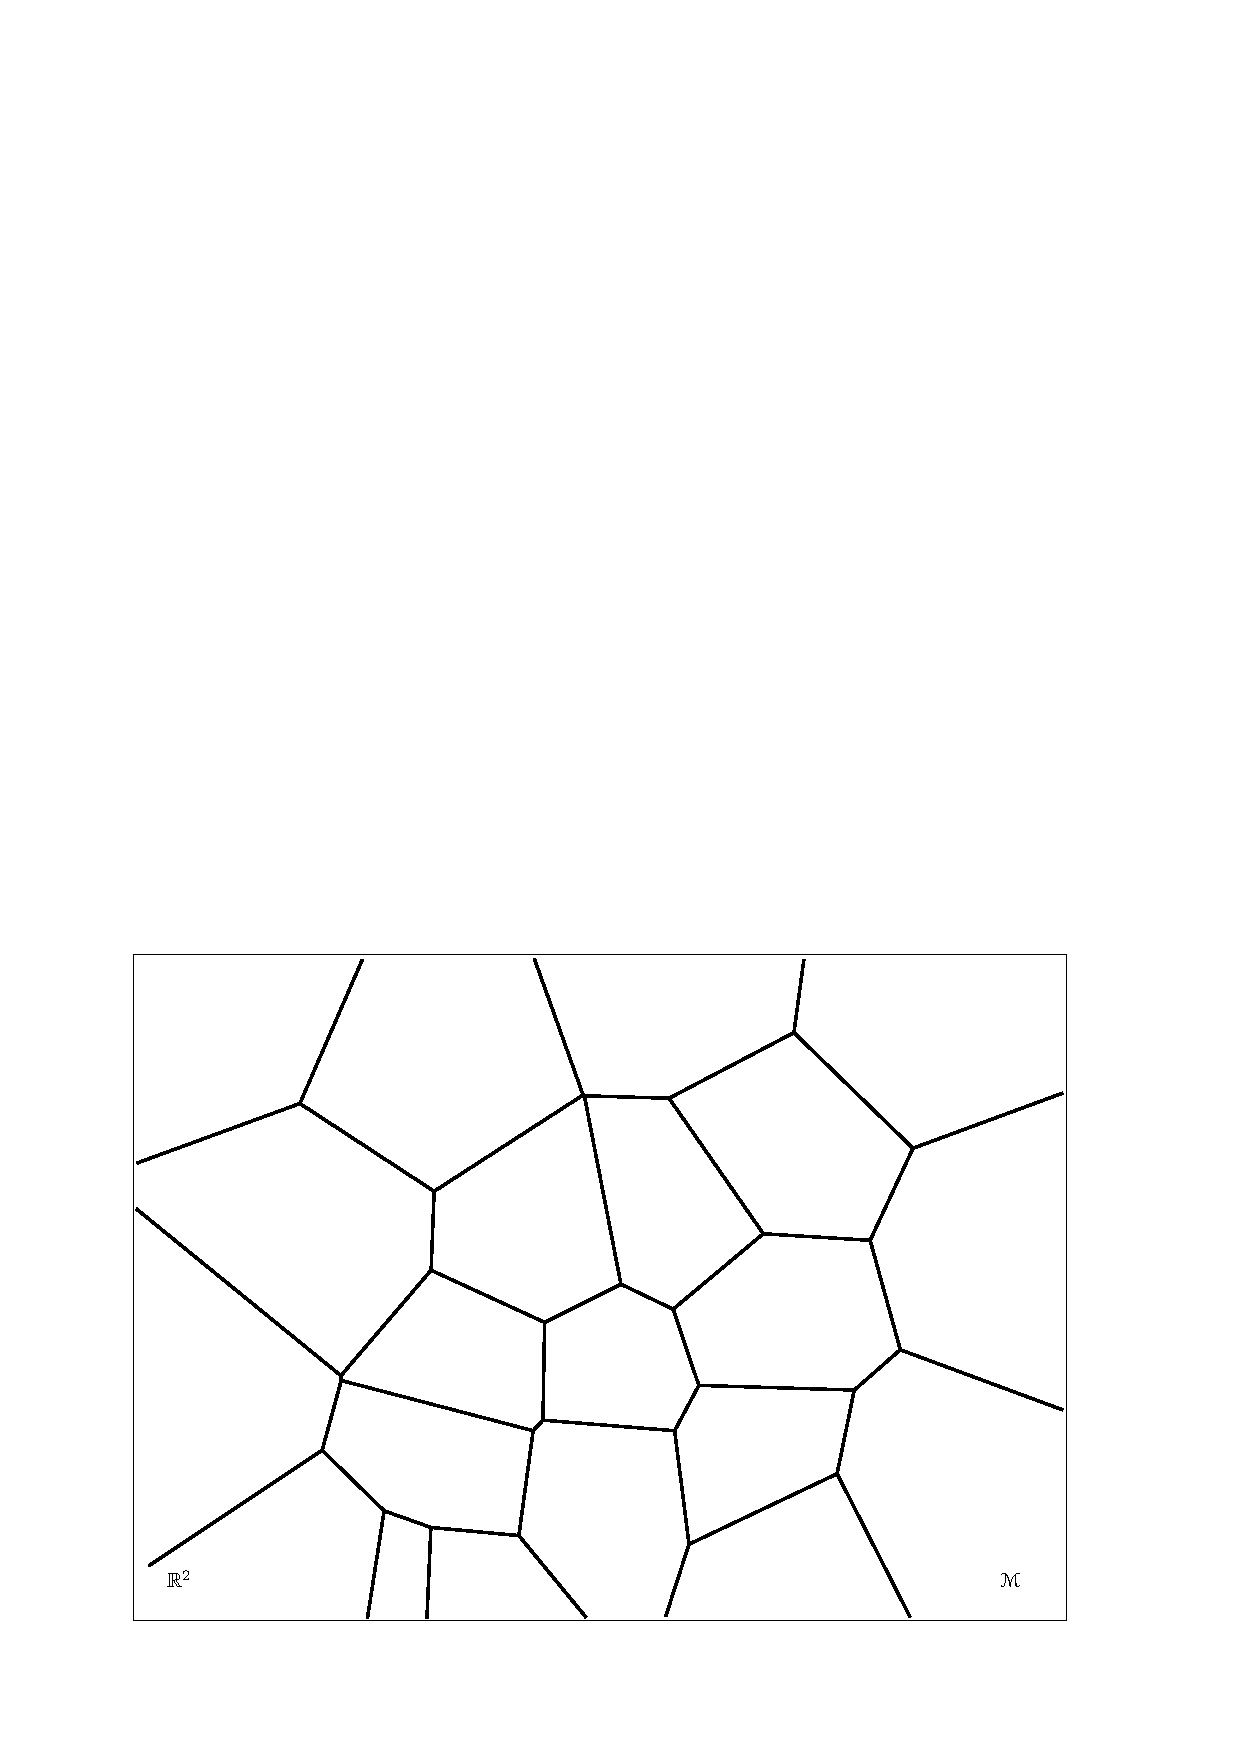
\includegraphics[height=120pt,page=1]{approx_diagram}%
\end{center}
\end{figure}
\begin{itemize}
\item \sout{How many distinct matchings appear in $\cost^*(t)$?}
\item What is the combinatorial complexity of $\M$?
\end{itemize}
\end{frame}

% main questions
\begin{frame}{Questions and prior results}
% second question is more general than the first: ``characterize cost^* for every translation''
\begin{enumerate}
\item {\large How quickly can we \alert{compute $t^*$}, a global minimum of $\cost^*(t)$?}
\item {\large What is the \alert{combinatorial complexity of $\M$}?}
	\begin{itemize}
	\pause
	\item \mycite{Rote 10}: in 1D, at most $m(n-m)+1$.
	\item \mycite{Ben-Avraham~{\etal} 14}: $O(n^2 m^{3.5}(e \ln m + e)^m)$ 
	\end{itemize}
\end{enumerate}
\vspace{20pt}
\begin{itemize}
\pause
\item Open to find $t^*$ in polytime, and whether $\M$ has polynomial complexity.
\pause
\item Approximation?
\end{itemize}
\end{frame}

% approximation lets us coarsen the diagram
\begin{frame}{Approximating $\M$ (1-dimensional)}
\begin{figure}
\begin{center}
\includegraphics<1>[width=0.8\textwidth,page=9]{lower_env}%
\includegraphics<2>[width=0.8\textwidth,page=10]{lower_env}%
\includegraphics<3>[width=0.8\textwidth,page=11]{lower_env}%
\includegraphics<4->[width=0.8\textwidth,page=12]{lower_env}%
%\includegraphics<6->[width=0.8\textwidth,page=6]{approx_diagram}%
\end{center}
\end{figure}
\end{frame}

\begin{frame}{Approximating $\M$ (2-dimensional)}
% function over t for each k matching
% cost*(t): the lower envelope
% vertical projection subdivides the plane
\begin{figure}
\begin{center}
\includegraphics<1>[width=0.8\textwidth,page=1]{approx_diagram}%
\includegraphics<2>[width=0.8\textwidth,page=2]{approx_diagram}%
\includegraphics<3>[width=0.8\textwidth,page=3]{approx_diagram}%
\includegraphics<4>[width=0.8\textwidth,page=4]{approx_diagram}%
\includegraphics<5->[width=0.8\textwidth,page=5]{approx_diagram}%
%\includegraphics<6->[width=0.8\textwidth,page=6]{approx_diagram}%
\end{center}
\end{figure}
\end{frame}

% take away: approximation gives polynomial solutions to both
\begin{frame}{Our results (approximation helps)}
% what is the combinatorial complexity of M?
%	we can construct an /approximate/ diagram ~M with polynomial size
%	each cell \tau of ~M has an associated matching M_\tau, \cost(M_\tau) approximates \cost*(t) for all t \in \tau
% can we compute t*, the minimum point of cost*(t)?
%	polytime algorithm by traversing all cells of ~M
\begin{enumerate}
\item {\large How quickly can we \alert{compute $t^*$}, a global minimum of $\cost^*(t)$?}
	\begin{theorem}
	In $\poly(m, n, \eps^{-1})$ time, can compute a $(1+\eps)$ \\
	\alert{approximation to $\cost^*(t^*)$} by exploring the faces of $\tildeM$.
	\end{theorem}
\item {\large What is the \alert{combinatorial complexity of $\M$}?}
	\begin{theorem}
	In $\poly(m, n, \eps^{-1})$ time, can construct a $(1+\eps)$
	\alert{approximate diagram} $\tildeM$ of complexity
	$O(n\eps^{-2}\log\eps^{-1})$.
	\end{theorem}
\end{enumerate}
\end{frame}

% result's strategy
\begin{frame}{Overview}
\begin{enumerate}
%\item We prove a \alert{Lipschitz property} for $\cost^*(t)$ over $t$.
%\pause
\item The set of \alert{point-to-point translations} give a constant
	approximate diagram of size $mn$.
\pause
\item Using exponential grids, constant $\rightarrow$ \alert{$(1+\eps)$ approximation}
	of size $O(mn\eps^{-2}\log\eps^{-1})$.
\pause
\item Reduce size to $O(\alert{n}\eps^{-2}\log\eps^{-1})$ by clustering.
\end{enumerate}
\end{frame}

% Lipschitz property --> point-to-point translations
\begin{frame}{Point-to-point translations}
% originally used by Cabello for for EMD under translations
% punchline: Vor(T) is constant approximate diagram!
\begin{itemize}
\item \alert{Point-to-point translations} \mycite{Cabello~{\etal} 08}:
	$T \coloneqq \{t_{ba} = (b - a) \mid a \in A, b \in B\}$
\begin{figure}
\begin{center}
\includegraphics<1>[width=0.6\textwidth,page=1]{point-to-point}%
\includegraphics<2>[width=0.6\textwidth,page=2]{point-to-point}%
\includegraphics<3>[width=0.6\textwidth,page=3]{point-to-point}%
\includegraphics<4>[width=0.6\textwidth,page=4]{point-to-point}%
\includegraphics<5>[width=0.6\textwidth,page=5]{point-to-point}%
\includegraphics<6>[width=0.6\textwidth,page=6]{point-to-point}%
\includegraphics<7>[width=0.6\textwidth,page=7]{point-to-point}%
\includegraphics<8>[width=0.6\textwidth,page=8]{point-to-point}%
\includegraphics<9->[width=0.6\textwidth,page=9]{point-to-point}%
\end{center}
\end{figure}
\item<10-> Enough to look at the optimal matching of each $t_{ba} \in T$.
\end{itemize}
\end{frame}

% voronoi diagram of point-to-points
\begin{frame}{$O(1)$-approximate diagram from point-to-point translations}
\begin{figure}
\begin{center}
\includegraphics<1>[width=0.7\textwidth,page=9]{point-to-point}%
\includegraphics<2>[width=0.7\textwidth,page=10]{point-to-point}%
\includegraphics<3>[width=0.7\textwidth,page=11]{point-to-point}%
\includegraphics<4>[width=0.7\textwidth,page=12]{point-to-point}%
\includegraphics<5->[width=0.7\textwidth,page=13]{point-to-point}%
\end{center}
\end{figure}
\begin{itemize}
\item<6-> $\tildeM$ is a constant-approximate diagram of size $\abs{T} = mn$.
\end{itemize}
\end{frame}

% constant --> (1+eps)
\begin{frame}{$O(1)$ $\rightarrow$ $(1+\eps)$ approximation}
% grid cell width 2^i cost^*(t_0)
% resulting complexity is O((mn/\eps^2) \log(1/\eps))
\begin{figure}
\begin{center}
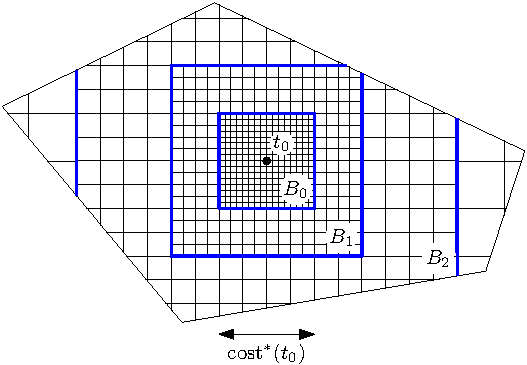
\includegraphics[width=0.5\textwidth,page=1]{nested-grid-crop}%
\end{center}
\end{figure}
\begin{itemize}
\item $(1+\eps)$ approximate diagram of size
	$O(\abs{T}\eps^{-2}\log\eps^{-1}) = O((mn)\eps^{-2}\log\eps^{-1})$
\end{itemize}
\end{frame}

% compressing ~M further
\begin{frame}{Near-linear size: clustering $T$}
% any O(1) approx is fine to apply the constant --> (1+eps) transformation
% cluster T? how to ensure cluster radius small wrt cost*(t)?
% here: reduce the size O(mn) to O(mn/k)
\begin{itemize}
\item Any $O(1)$ approx. diagram is enough for the $(1+\eps)$ diagram.
\item Partition $T$ into clusters of size at least $m/2$.
\begin{figure}
\begin{center}
\includegraphics<1>[width=0.7\textwidth,page=10]{point-to-point}%
\includegraphics<2>[width=0.7\textwidth,page=9]{point-to-point}%
\includegraphics<3>[width=0.7\textwidth,page=14]{point-to-point}%
\includegraphics<4>[width=0.7\textwidth,page=15]{point-to-point}%
\includegraphics<5>[width=0.7\textwidth,page=16]{point-to-point}%
\includegraphics<6>[width=0.7\textwidth,page=17]{point-to-point}%
\includegraphics<7>[width=0.7\textwidth,page=18]{point-to-point}%
\includegraphics<8>[width=0.7\textwidth,page=19]{point-to-point}%
\includegraphics<9>[width=0.7\textwidth,page=20]{point-to-point}%
\includegraphics<10>[width=0.7\textwidth,page=21]{point-to-point}%
\includegraphics<11>[width=0.7\textwidth,page=22]{point-to-point}%
\includegraphics<12>[width=0.7\textwidth,page=23]{point-to-point}%
\includegraphics<13>[width=0.7\textwidth,page=24]{point-to-point}%
\includegraphics<14>[width=0.7\textwidth,page=25]{point-to-point}%
\includegraphics<15>[width=0.7\textwidth,page=26]{point-to-point}%
\includegraphics<16->[width=0.7\textwidth,page=27]{point-to-point}%
\end{center}
\end{figure}
\item<17-> Reduces diagram size from $mn \rightarrow O(n)$.
\end{itemize}
\end{frame}

% open questions
\begin{frame}{Open questions}
% is the complexity of the exact minimization diagram polynomial? for p=2?
% approximate diagrams for rotations? rigid transforms?
\begin{enumerate}
\item Is the complexity of $\M$ polynomial?
\item Approximate diagrams for rotations? Rigid transforms?
\end{enumerate}
\end{frame}

% end slide
\begin{frame}{The End}
\begin{center}
	Thank you.
\end{center}
\end{frame}

%\begin{frame}[allowframebreaks]{Citations}
%\tiny
%\bibliography{ref}
%\bibliographystyle{alpha}
%\end{frame}


\end{document}
